\section{Tema 3: Atom og bindinger}
\label{tema3}

\begin{table}[!htb]
    \centering
    \caption{Samtale punkter tema 3}
    \begin{tabular}{|c|c|c|r|}
      \hline
      1 & Kvantebrønn i 3D (partikkel i boks) &  \autoref{sec:tema3_1} & \cellcolor{blue}\quad\quad \\
      \hline 
      2 & Degenerasjon & \autoref{sec:tema3_2} & \cellcolor{blue} \\
      \hline
      3 & Hydrogenatomet & \autoref{sec:tema3_3} & \cellcolor{blue} \\
      \hline
      4 & Det periodiske systemet og Elektronkonfigurasjon & \autoref{sec:tema3_4} & \cellcolor{blue} \\
      \hline 
      5 & Bindinger i faste stoffer & \autoref{sec:tema3_6} & \cellcolor{green} \\ 
      \hline
      6 & Dobbel kvantebrønn & \autoref{sec:tema3_7} & \cellcolor{blue} \\
      \hline
      7 & Det interatomære potensiale & \autoref{sec:tema3_8} & \cellcolor{blue} \\
      \hline
    \end{tabular}
    \label{tab:samtalePunkt_tema1}
\end{table}

\subsection{Kvantebrønn i 3D (partikkel i boks)}
\label{sec:tema3_1}
Vi beveger oss fra å jobbe i 1D til 3D, men løsningen på partikkel i boks har lignende løsning som partikkel i 1D brønn. \autoref{eq:1D-Sol} viser løsningen på problemet i 1D.

\begin{equation}
\label{eq:1D-Sol}
    \bigg[
    \psi_n(x) = \sqrt{\frac{1}{a}}sin\bigg(\frac{n\pi x}{L}\bigg),
    \;E_n = \frac{n^2\pi^2\hbar^2}{2ma^2}
    \bigg]
\end{equation}

I 3D legger vi til litt komplekst, vi antar nå vi har en kube, så alle veggene er $a$ lange i $x$-, $y$- og $z$-retning. Dette gir \ref{eq:3D-sol}

\begin{equation}
    \label{eq:3D-sol}
    \psi(x,y,z) = \sqrt{\frac{2^3}{a^3}}
    sin\bigg(\frac{n_x\pi x}{a}\bigg)
    sin\bigg(\frac{n_y\pi y}{a}\bigg)
    sin\bigg(\frac{n_z\pi z}{a}\bigg)
\end{equation}

og energien kommer ut på formen 

\begin{equation}
    \label{eq:3D-energi}
    E_{n_xn_yn_z} = \frac{\pi^2\hbar^2}{2ma^2}
    \bigg(
    n_x^2+n_y^2+n_z^2
    \bigg)
\end{equation}

I ligning \ref{eq:3D-energi} står $n_i$ for kvantetall, altså kun positive heltall fra $1$ og oppover. Ulike kombinasjoner kan produsere sammen energi, men de ulike kombinasjonene produserer samme energi kan de ikke ha lik bølgefunksjon $\psi(x,y,z)$, dette ser vi siden $n_i$ inngår i sine respektive sinus funksjoner.

\subsection{Degenerasjon}
\label{sec:tema3_2}
\autoref{fig:degen_energi} viser oversikt over energitilstander med tilhørende kvantetall. Det er synlig at f.eks første energi nivå har vi at alle kvantetallene er $1$. Dette er ikke en degenerert tilstand, da det kun er en bølgefunksjon som korresponderer med energi nivået. En degenerert tilstand er definert som en tilstand der et system kan ha lik energi i flere konfigurasjoner av kvantetall, men ulike bølgefunksjoner. 

\begin{figure}[!htb]
    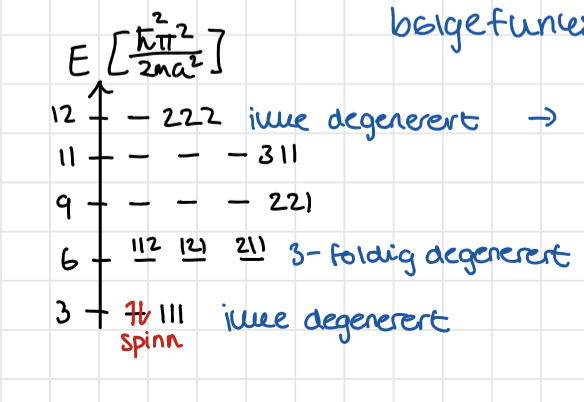
\includegraphics[width=0.9\textwidth]{Bilder/SamtaleTema3/3D partikkel i boks/degenererteTilstander.png}
    \caption{Oversikt over energitilstander og degenererte tilstander}
    \label{fig:degen_energi}
\end{figure}

Lengden på sidene av den 3D boksen er viktig, det er også symmetri når det kommer til degenerasjon. Om alle sidene hadde vært forskjellige hadde \textbf{alle} energinivåene vært separert. \color{red} Degernasjon er et resultat av symmetri i systemet. \color{black}

Som man ser fra figur \ref{fig:degen_energi}, ligger det to piler på det laveste energi nivået, grunntilstanden om man vil. Disse pilene representerer spinn. Elektroner har en kvantemekanisk egenskap som gjør at de spinner, det finnes kun to spinn konfigurasjoner, spinn opp og spinn ned. Dette fører oss til et resultat som Wolfgang Pauli postulerte i 1925, det fikk navnet Paulis eksklusjonsprinsipp.

\begin{definition}
    \textbf{Pauls ekslusjonsprinsipp}: To eller flere fermioner kan ikke være i samme kvantetilstand samtidig
\end{definition}

Dette vil si at to elektroner ikke kan inneha samme bølgefunksjon, eller spinn opp/ned. Definisjonen sier fermioner, for dette kurset er det verdt å merke at et elektron er et fermion. 

Resulatet av prinsippet fører til at elektroner må fylle opp høyere og høyere energinivåer siden det ikke er ''plass''. Dette betyr også at en bevegelsesmengde kan være opptatt.

\subsection{Hydrogenatomet}
\label{sec:tema3_3}
Hydrogenatomet er det enkleste atomet i det periodiske system. Hydrogenatomet er bestående av en kjerne med en positiv ladning, og et elektron i skalet. Det er Coulum-krefter som holder de to sammen. Kvantisering gjør at det bare kan velge noen spesifikke energinivå.

Potensialet til hydrogenatomet må være rotasjonssymmetrisk uten endelige grenser. Det skal da være sterkere krefter jo nærmere kjernen man kommer. Det vil si at det kreves mer å ''ta'' et elektron som sitter i grunntilstand ($n=1$). \autoref{fig:hydro-pot} viser hydrogenatomet sitt potensialet.

\begin{figure}[!htb]
    \centering
    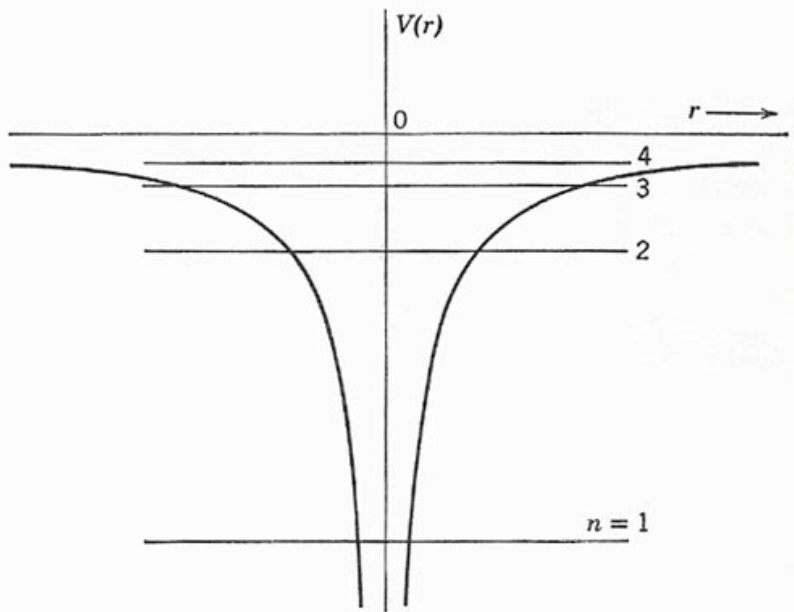
\includegraphics[scale=0.8]{Bilder/SamtaleTema3/Hydrogenatomet/hydrogenPot.png}
    \caption{Representasjon av potensialet til et hydrogenatom, r er radialle avstanden fra massesenteret.}
    \label{fig:hydro-pot}
\end{figure}

Hydrogenatomet har 3 kvantetall ($n$,$l$,$m$), bølgefunksjonen med polare koordinater kan derfor representeres som

\begin{equation}
    \psi_{lnm}(r,\theta,\phi)
\end{equation}

Der $n$ er det prinsipielle kvantetallet, $l$ er kvantetallet for angulær bevegelsesmengde (orbital kvantetall) og $m$ er det magnetiske kvantetallet.

\color{red}

\begin{itemize}
\centering
    \item $n$ relaterer til total energi
    \item $l$ relaterer til drivmoment (spinn)
    \item $m$ relaterer til z-komponenten til drivmomentet (hvilken retning den spinner)
\end{itemize}
\color{black}

\newpage
Kvantetallene kan inneha verdiene 

\begin{equation*}
    \begin{split}
        n &= 1, 2, 3, ...\\
        l &= 0, 1, 2, 3, ..., n-1\\
        m_l &= -l, -(l-1), ..., 0, ..., l
    \end{split}
\end{equation*}

En tilstand til hydrogenatomet med kvantetall $n=1$,$l=0$ og $m=0$ gir
$\psi_{100}$ osv. Dette gjelder kun for systemer med et elektron. 

For et system med et elektron vil energi nivå diagramet se ut som \href{https://www.google.com/search?q=energy+level+diagram+for+hydrogen&sca_esv=779b01740ca52ec5&sca_upv=1&rlz=1C5CHFA_enNO829NO829&udm=2&biw=1680&bih=904&sxsrf=ACQVn09akSWsMLxftMzmPMdTNcY0gxBSJA%3A1714049752819&ei=2FIqZpLKMbjPwPAP7-qYwAQ&oq=Energy+level+diagr&gs_lp=Egxnd3Mtd2l6LXNlcnAiEkVuZXJneSBsZXZlbCBkaWFncioCCAEyBRAAGIAEMgoQABiABBhDGIoFMgUQABiABDIKEAAYgAQYQxiKBTIFEAAYgAQyBRAAGIAEMgUQABiABDIFEAAYgAQyBRAAGIAEMgUQABiABEiVO1DKBVikKHAGeACQAQCYAfsBoAH7DaoBBjE2LjQuMbgBA8gBAPgBAZgCGKAC5A7CAgQQIxgnmAMAiAYBkgcGMTkuNC4xoAf_dw&sclient=gws-wiz-serp#vhid=NSb9L5eew_qdbM&vssid=mosaic}{Her}. Men når atomett har flere elektroner vil diagrammet forskyves litt, og det vil bli færre degenererte states. 

Madelungs regel går ut på at fylling av energinivåer går fra lavest til høyest verdi av $n+l$. Når to orbitaler har samme verdi for $n+l$, vil den med lavest $n$ bli fylt først. 

\subsection{Det periodiske systemet og Elektronkonfigurasjon}
\label{sec:tema3_4}
Det er mulig at to elektron opptar en energitilstand, en med spinn opp og en med spinn ned, det vil si at det er plass til to elektron per orbital. Dette henger sammen med mengde elektroner i atomer av forskjellige typer.

Vi ser på edelgasser som et eksempel. Neon [$He$] består av $2S^22P^6$, vi ser at åtteregelen er oppfylt i neon sitt tilfelle, skriver bare det i tillegg til forrige edelgass. Edelgaser har en ekstra stabil konfigurasjon.

Sannsynligheten for å finne et elektron i 1$S$-tilstanden har en radiell fordeling, altså en funksjon av avstanden fra sentrum. 

\begin{figure}[!htb]
    \centering
    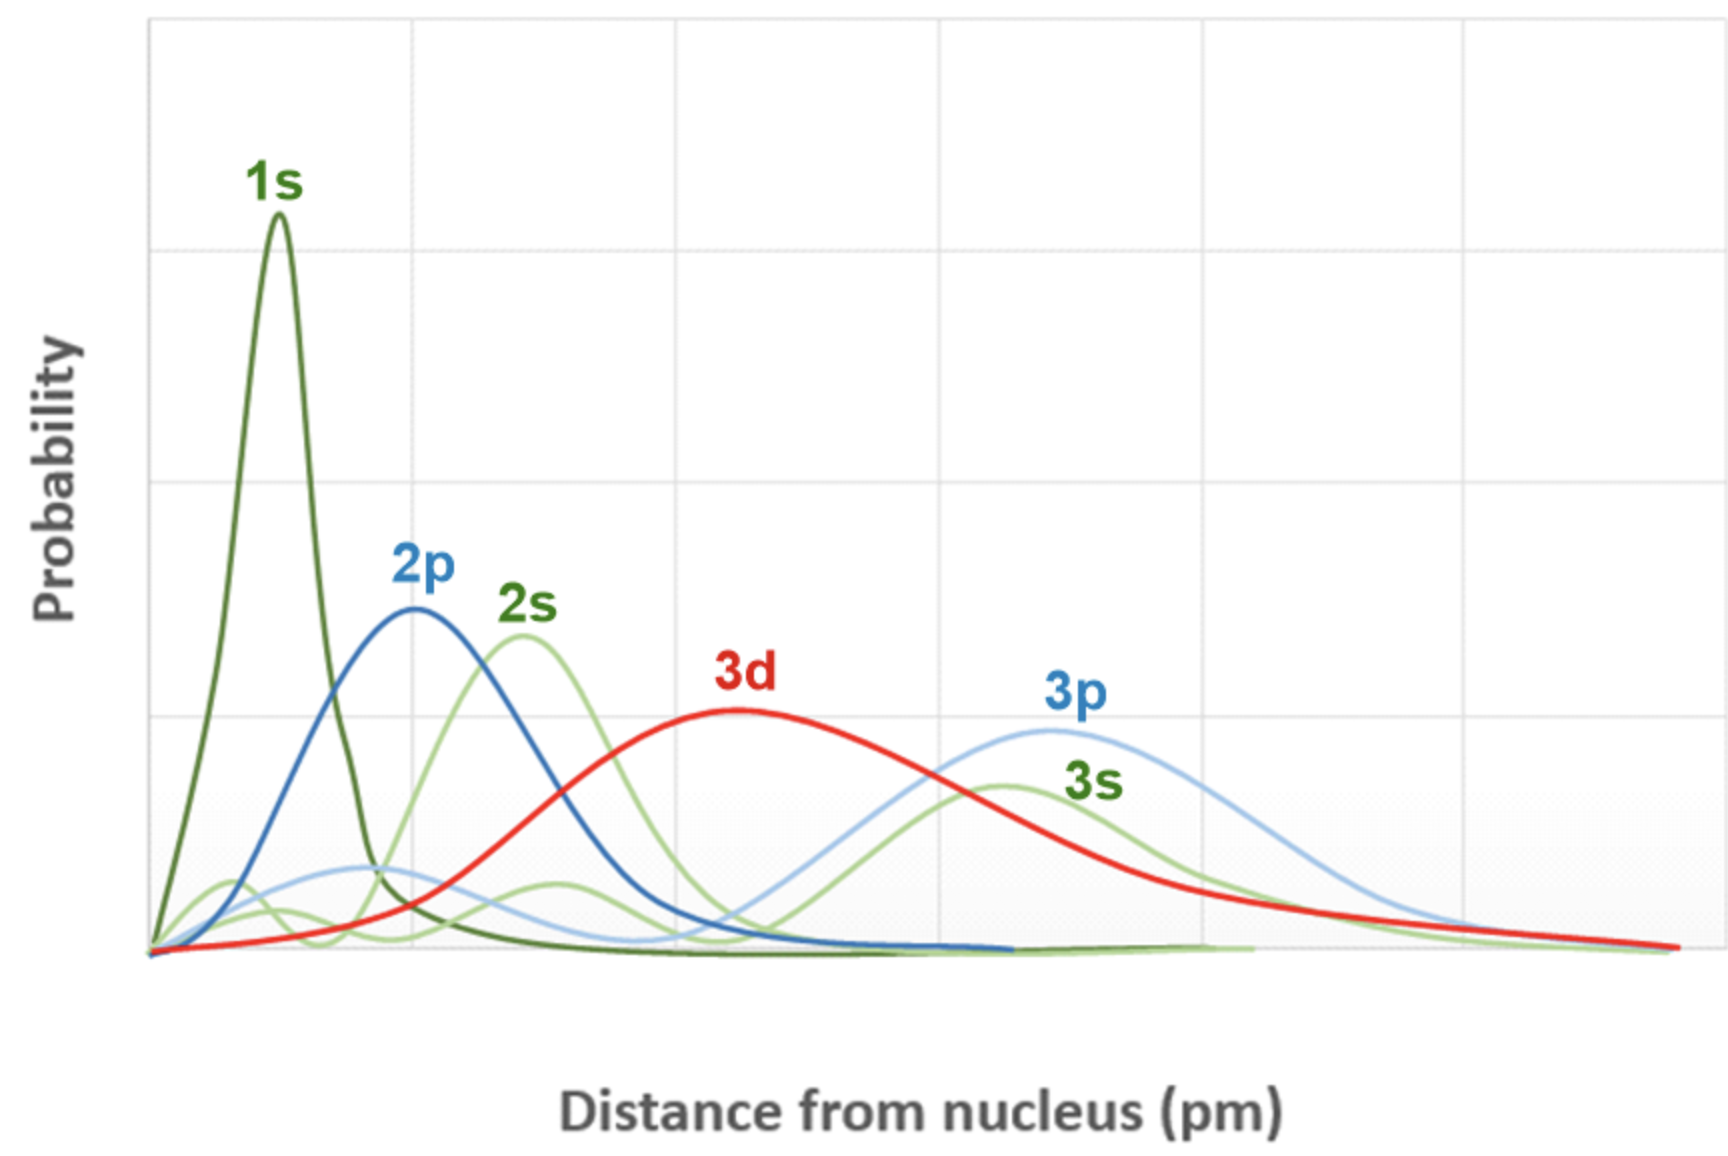
\includegraphics[scale=0.35]{Bilder/SamtaleTema3/InterPotens/radiellAvstand.png}
    \caption{Tilnærmet null sannsynlighet for noen av orbitalene å ha elektrone ved kjernen, vi ser at snitt verdien for avstand øker med økende orbital.}
    \label{fig:avstand}
\end{figure}

Orbitaler er nesten som en kompakt kule når alle ligger samlet og er flle, så et elektron som ligger i neste skall er ''ganske'' fritt.

Hund's regel sier at ''antall uparede elektroner (spinn opp/ned) er maksimert'' og ''Diisse uparede elektronene har egenskapen ''paralell spinn'', som medfører max total spinn i den ytterste orbitalen.''
Dette er fordi det å oppnå ulike orbitaler er ønskelig og energimessig, siden det reduserer gjensidig frastøtning og skjerming av atomkjernen. Med parallel spinn, har disse $e^-$ en null prosent sannsynlighet for å befinne seg i samme orbital, dette oppfyller Paulis eksklusjonsprinsipp.

\begin{figure}[!htb]
    \centering
    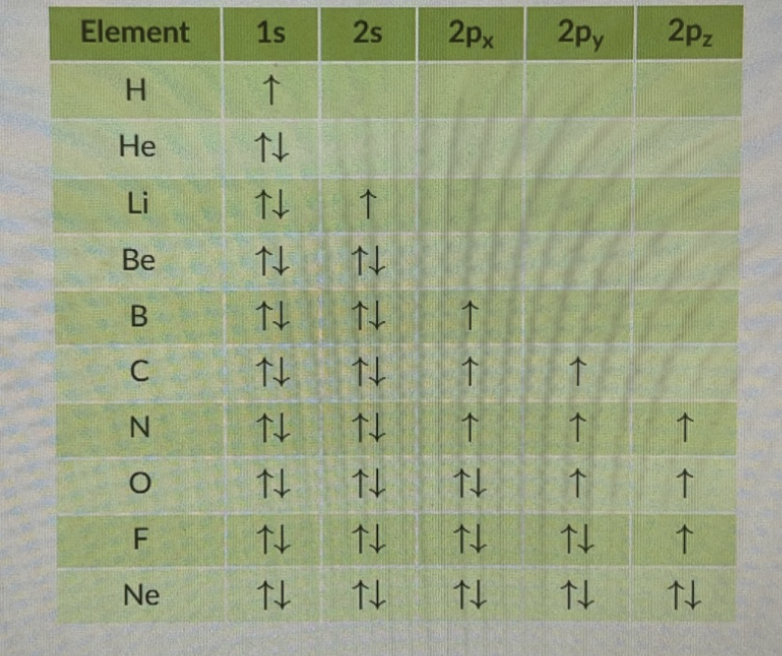
\includegraphics[scale=1]{Bilder/SamtaleTema3/box-arrow.png}
    \caption{Boks-pil diagram for de 10 første elementene i det periodiske system}
    \label{fig:box-arrow}
\end{figure}


\subsection{Bindinger i faste stoffer}
\label{sec:tema3_6}
Vi skal se på 3 viktige binder i denne underseksjonen, det er Ioniske bindinger, Metalliske bindinger og Koavalente bindinger.

Ioniske bindinger er veldig sterke bindinger, de er gode isolatorer fordi elektronkonfigurasjonen er veldig stabil. Bindingen er melom to ioner med motsatt ladning. Sterkere forskjell i elektronegativiteten gir en sterkere binding. I en ionisk binding er det ingen frie elektroner, dette gjør det som sagt til en dårlig leder, men en god isolator. vanlig sammensetning er ett atom med ett elektron i valensskallet, med ett som mangler ett for å oppnå edelgass konfigurasjon.

\begin{figure}[!htb]
    \centering
    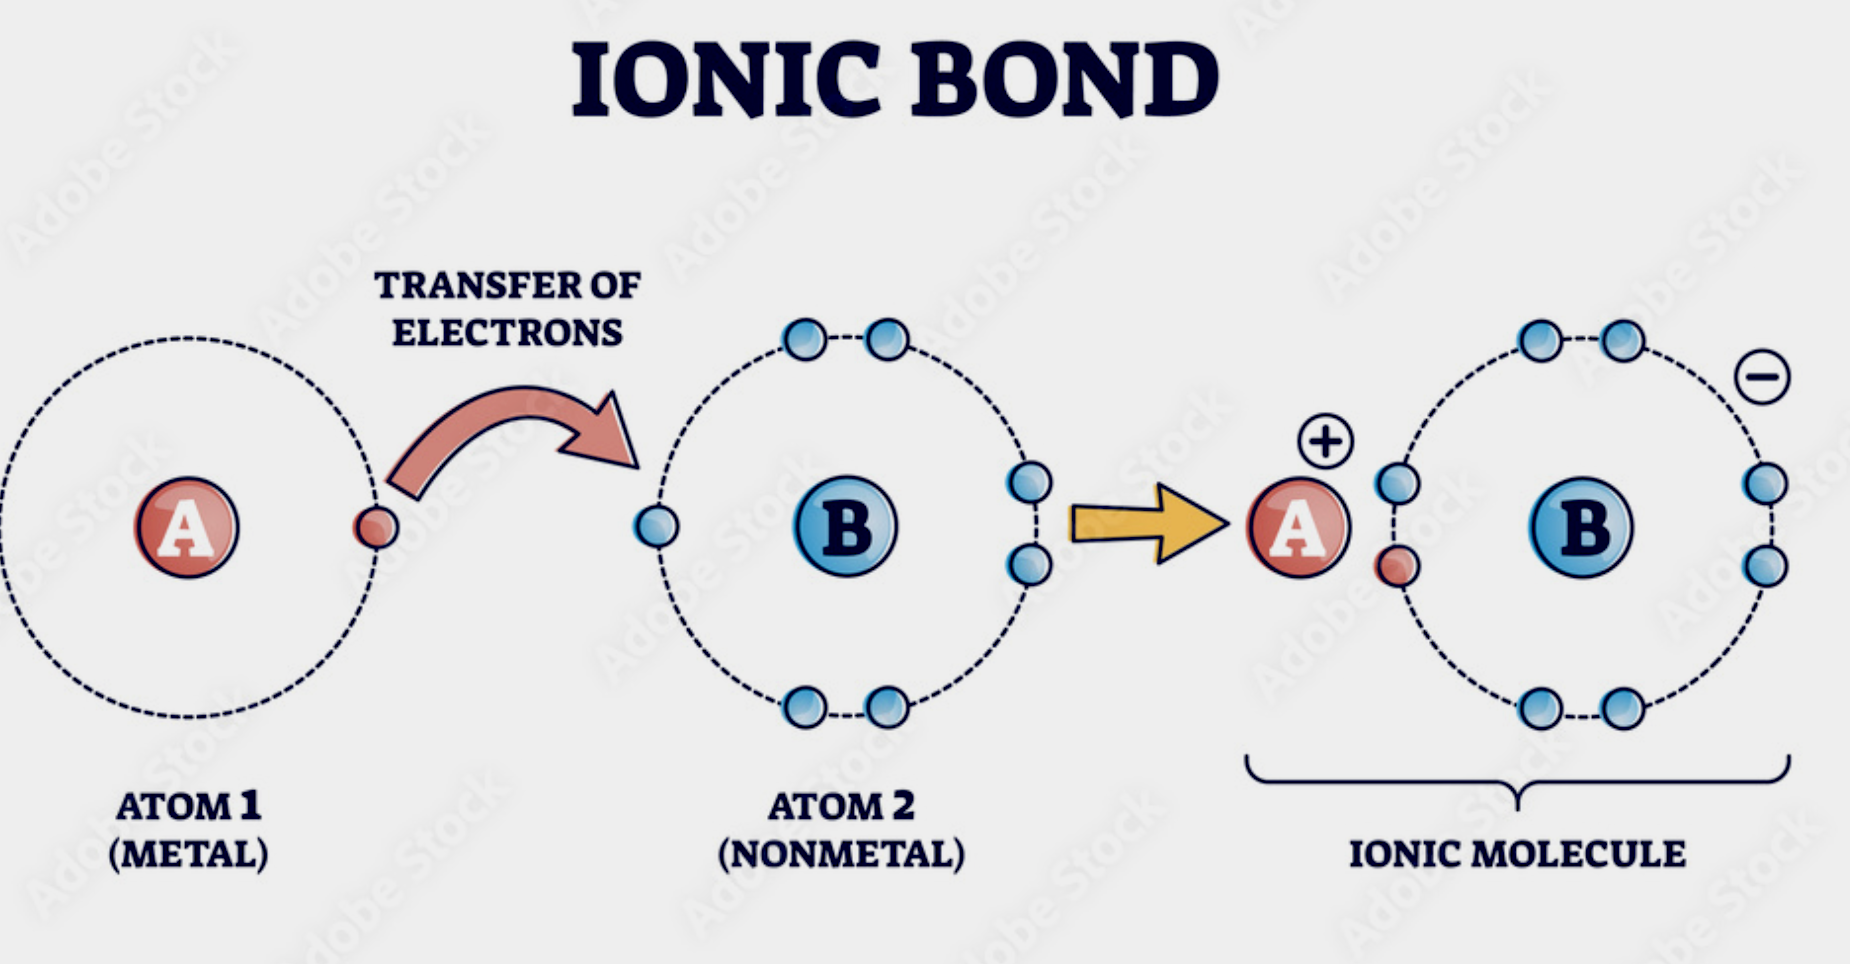
\includegraphics[scale=0.4]{Bilder/SamtaleTema3/Bindinger/ionic.png}
    \caption{Ionisk binding}
    \label{fig:ione}
\end{figure}

Metalliske bindinger er bindinger som oppstår i metaller, de er typisk gode til å lede. Bindingene oppstår mellom atomer med lav elektronegativitet, det holder metaller sammen. Man sier ofte at metall atomene er omgitt av et elektronhav der atomer ikke holdes fast av de andre atomene, men av elektronsjøen. Metaller er gode ledere nettop pga. dette, elektronene er ikke fastbundne, så de har en relattivt fri flyt. Dette er bindinger som ikke er like sterke som iioniske og koavalente bindinger. 

\begin{figure}[!htb]
    \centering
    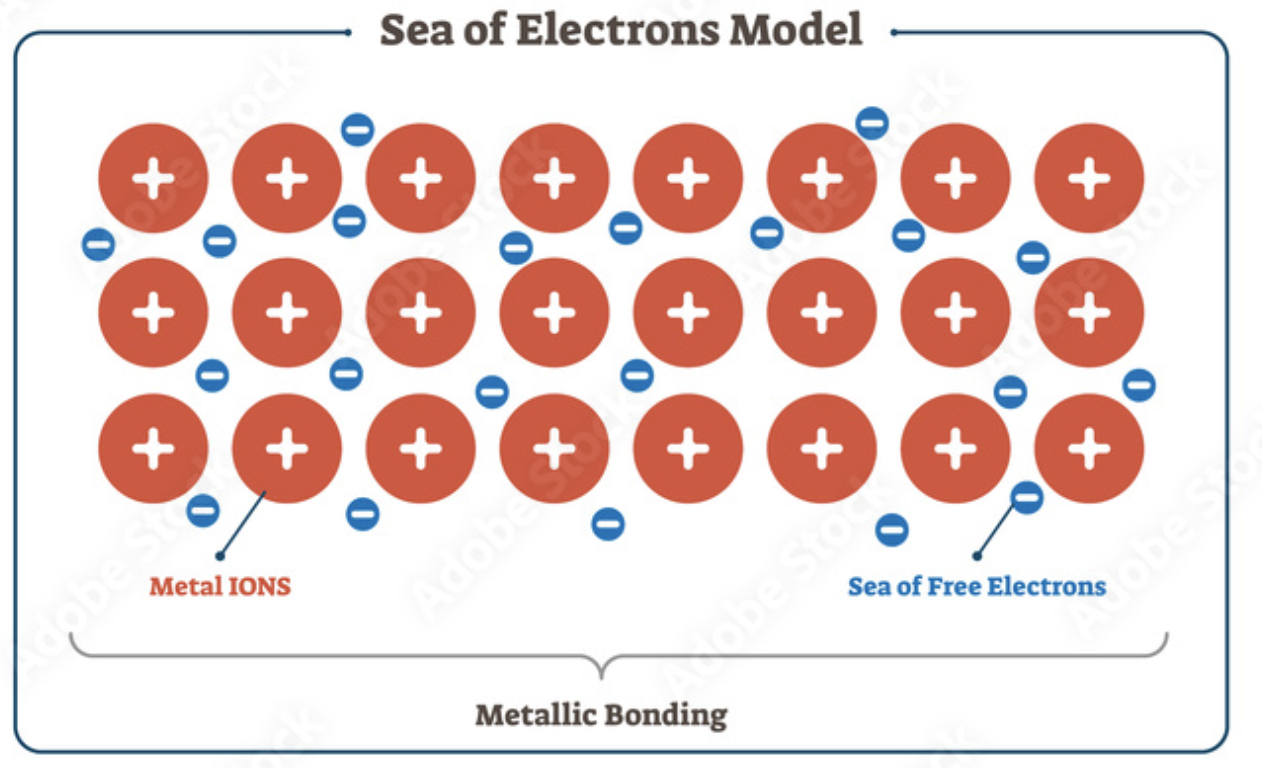
\includegraphics[scale=0.4]{Bilder/SamtaleTema3/Bindinger/metallic.png}
    \caption{Elektronsjø representasjon av metalliske bindinger}
    \label{fig:metallisk}
\end{figure}

Koavalente bindinger, oppstår ofte i halvledere, de er bistabile mellom å være en leder og en isolator. Koavalente bindingener oppstår mellom to molekyler som deler et elektronpar. Dette kan være enkelt, dobbelt eller trippelbinding. Det har dårlig ledningsevne da elektronene for det meste er lokalisert mellom atomene. Det er sterke bånd, men med kort båndlengde. 

Koavalente bindinger oppstår ofte når alle mangler ett eller flere elektron for edelgasskonfigurasjon, ved å bryte mange bindinger vil det lede bedre og bedre. 

\begin{figure}[!htb]
    \centering
    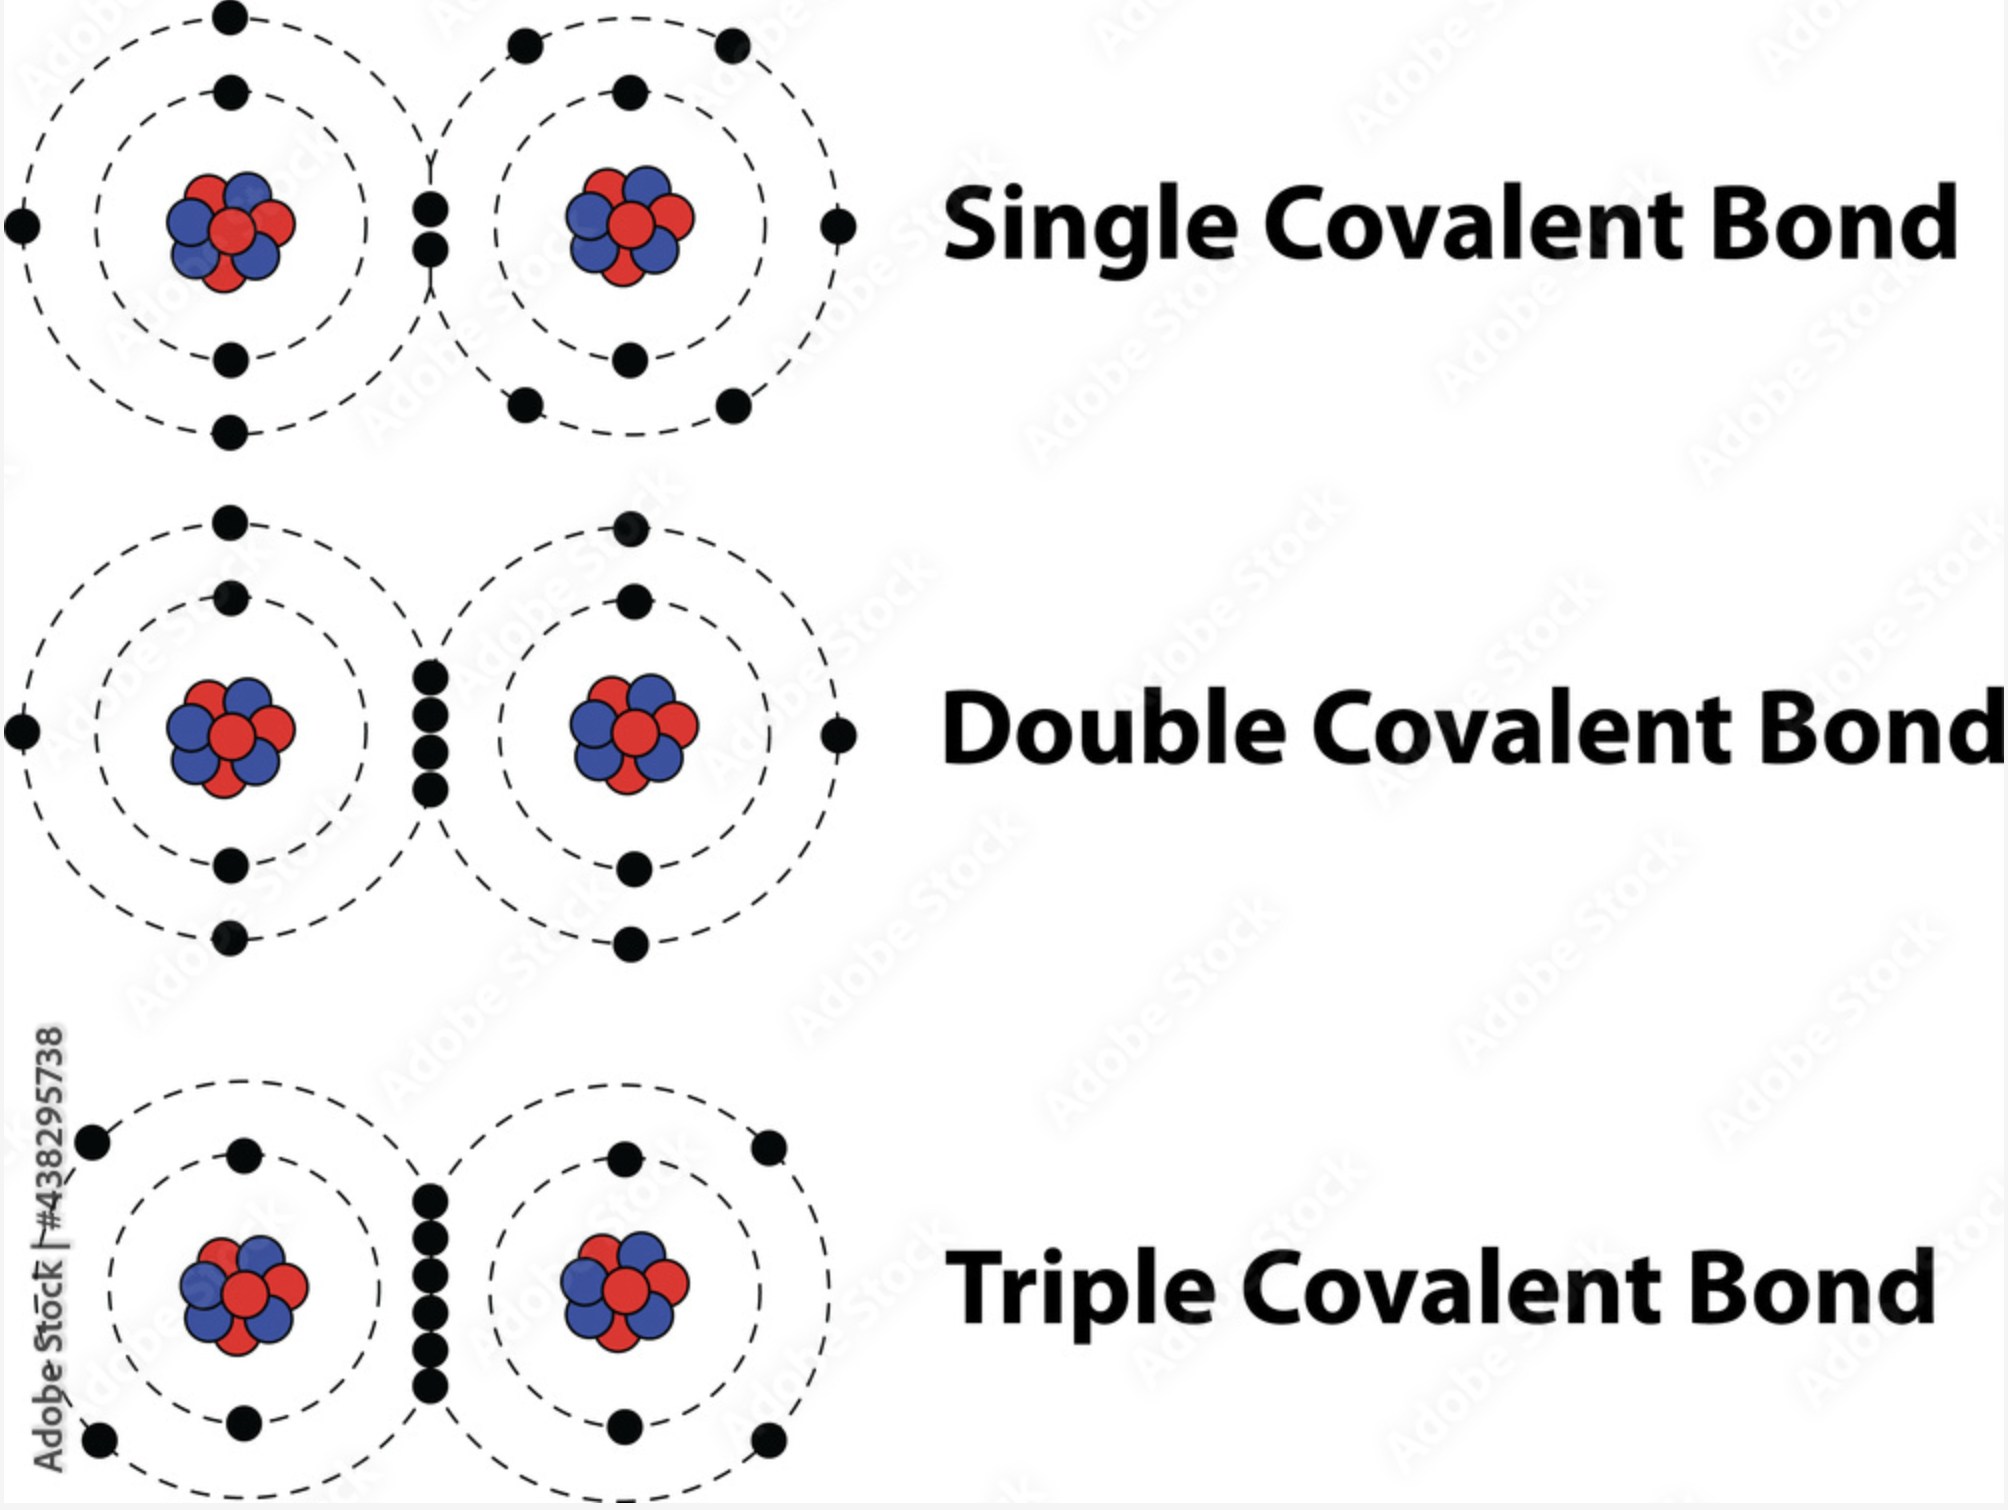
\includegraphics[scale=0.3]{Bilder/SamtaleTema3/Bindinger/covalent.png}
    \caption{enkel, dobbel og trippel covalent binding}
    \label{fig:cov}
\end{figure}

\subsection{Dobbel kvantebrønn}
\label{sec:tema3_7}
Vi har til nå sett på kvantebrønn i 1D, dette har vi sett på som en forenklet modell av hydrogenatomet, men vi vil gjerne introdusere mer kompleksistet så vi kan jobbe med mer enn bare et elektron og et proton. Vi legger til et proton i kjernen til Hydrogen atomet og får $H_2^+$, dette kan vi se på som to brønner som står ved siden av hverandre. 

Ved å føre to brønner sammen, der begge er i grunntilstand får vi figur \ref{fig.dobbelB}

\begin{figure}[!htb]
    \centering
    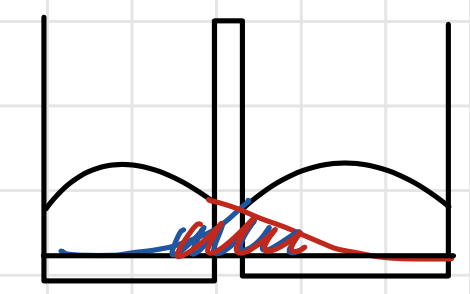
\includegraphics[scale=1]{Bilder/SamtaleTema3/DobbelBrønn/dobbelBrønn.png}
    \caption{To enkelt brønner lagt sammen til en dobbelbrønn, $\psi_1$ og $\psi_2$. Det skraverte området er en del av løsningen som bryter med Paulis eksklusjonsprinsipp.}
    \label{fig:dobbelB}
\end{figure}

Siden atomene er tett på hverandre, og barrieren mellom dem ikke er uendelig høy eller ''langt unna'', kan bølgefunksjonen tunnellere gjennom og lekke over til motsatte side. Problem når bølgefunksjonene tar pass på sted pga. Paulis eksklusjonsprinsipp.

Vi har hvertfall en superposisjon av tilstandene

\begin{equation*}
    \begin{split}
    \psi_B &= \psi_1 + \psi_2\\
    \psi_A &= \psi_1 - \psi_2
    \end{split}
\end{equation*}

Disse er begge gyldige løsninger på SL. Å sette sammen to atomer slik endrer grunntilstanden (de gror sammen, danner enten en sum eller differanse). Den som har lavest energi og som dermed blir den nye grunntilstanden er $\psi_B$ siden den har mindre krumming, den dobbelderiverte er mindre. \autoref{fig:solDobbel} viser hvordan grunntilstanden og første eksiterte tilstand vil se ut.

\begin{figure}[!htb]
    \centering
    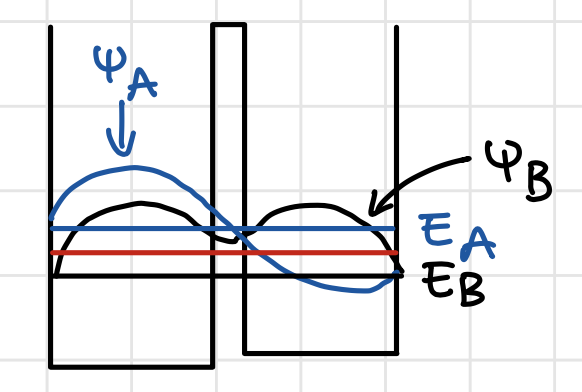
\includegraphics{Bilder/SamtaleTema3/DobbelBrønn/solDobbel.png}
    \caption{Røde linjen er energien til den gamle bølgefunksjonen.}
    \label{fig:solDobbel}
\end{figure}

$\psi_B$ har subskriptet B da det står for bonding orbital, det er bølgefunksjonen som indikerer en binding mellom to atomer. Den senker $E$, mer gunstig for systemet å være her. Det ligner på et kovalent bånd.

$\psi_A$ har subskript A da det står for Anti bonding orbital, den hever energien og den har lav $|\psi_A|^2$ mellom atomene. 

Barriere har noe å si, jo høyere energinivåer desto lettere å tunnellere gjennom barrieren (mye lekkasje). Tilstandene med mindre energi ser en større barriere og sannsynligheten for at de tunnellerer er liten.

Lavt energinivå betyr at atomene er langt fra hverandre, høyere er da nærmere, og de har stor energi i forhold til høyden på brønnen, det vil si større lekkasje da det skal mindre til å tunnellere.

\subsection{Det interatomære potensiale}
\label{sec:tema3_8}
Det interatomære potensialet referer til den potensielle energien mellom to eller flere atomer. Den oppstår som følge av interaksjoner mellom de tilhørende partiklene som elektroner og protoner/nøytroner.

Oppsummert er det energien som to eller flere atomer har pga. en gjensidig tiltrekning/frastøtning. Potensialet påvirker hvordan atomer interagerer og bindes sammen.

\begin{figure}[!htb]
    \centering
    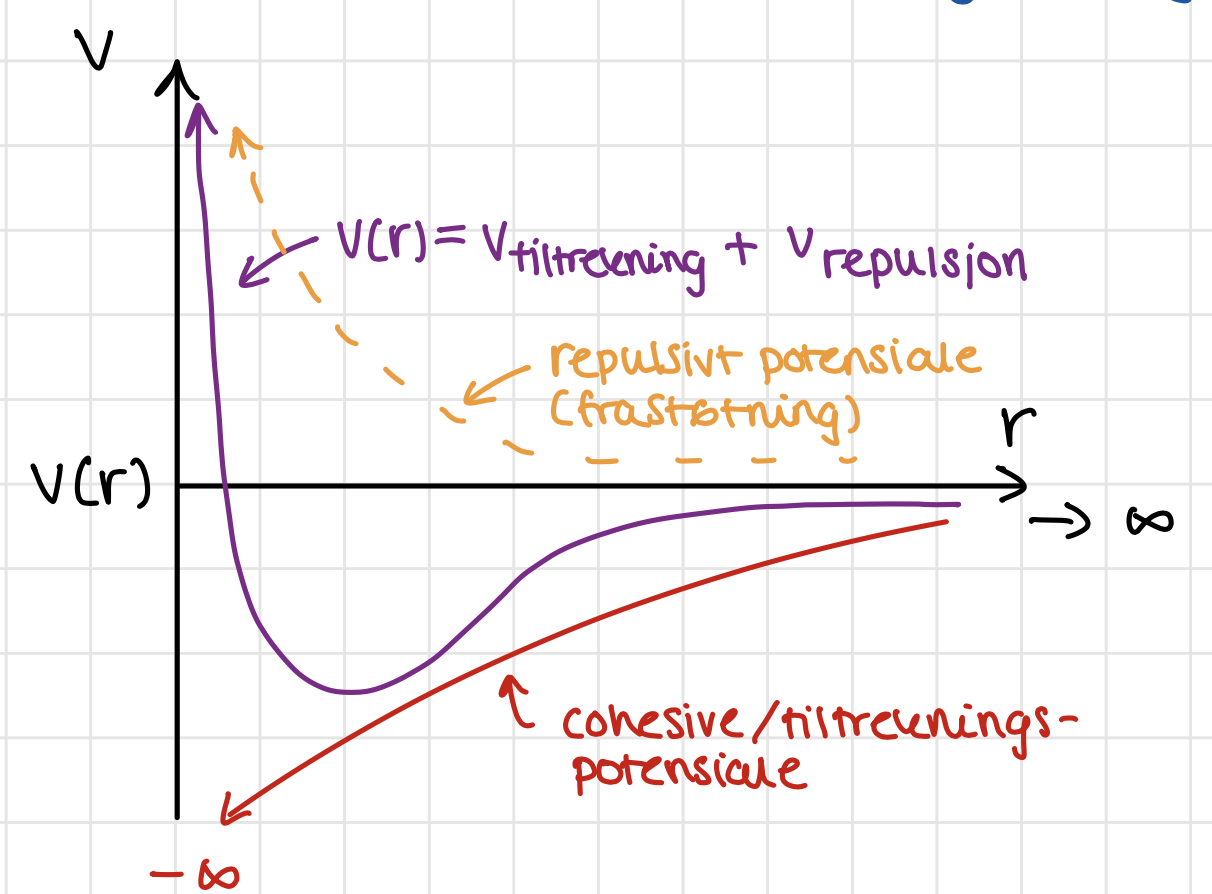
\includegraphics[scale=0.6]{Bilder/SamtaleTema3/InterPotens/Ipot.png}
    \caption{Interatomær energikurve for potensiell energi, en funksjon av den radielle avstanden $r$.}
    \label{fig:Ipot}
\end{figure}

Vi bruker $r$ i figur \ref{fig:Ipot} fordi vi antar at atomer og ioner er radielt symmetriske. Med det er $r$ avstanden mellom atomene. 

Det er mulig å si at to atomer langt unna hverandre ser hverandre, og vil i realiteten alltid påvirke hverandre, men den potensielle energien er tilnærmet null når man er langt unna. 

Tenker vi på atomer med ulike orbitaler, vil de ikke at orbitalene skal overlappe for mye, Dette er ofte forklart med Paulis eksklusjonsprinsipp, men essensielt så er det en energi som hindrer overlappen.

\newpage